%% Beamer theme to be used by LIP6 teams.
%% This is a skeleton file demonstrating
%% the use of the theme Frederiksberg version 2.2
%% with the UPMC visual guidelines applied.
%%
%% Version 1.1
%% May 19, 2012
%% by S�bastien Heymann <sebastien.heymann@lip6.fr>, http://sebastien.pro/
%% from LIP6 ComplexNetworks
%%
%% REQUIREMENTS:
%% - compile with pdflatex (tested on Windows7 with Texmaker 3.2)
%% - install http://matdat.life.ku.dk/LaTeX/Frederiksberg
%%
%% WARNINGS:
%% - load this file in ISO-8859-1 and keep using this encoding

%%*************************************************************************
%% Legal Notice:
%% Copyright (c) 2012 S�bastien Heymann <sebastien.heymann@lip6.fr>
%% 
%% Permission is hereby granted, free of charge, to any person obtaining a copy of 
%% this software and associated documentation files (the "Software"), to deal in the 
%% Software without restriction, including without limitation the rights to use, copy, 
%% modify, merge, publish, distribute, sublicense, and/or sell copies of the Software, 
%% and to permit persons to whom the Software is furnished to do so, subject to the 
%% following conditions:
%% 
%% The above copyright notice and this permission notice shall be included in all 
%% copies or substantial portions of the Software.
%% 
%% THE SOFTWARE IS PROVIDED "AS IS", WITHOUT WARRANTY OF ANY KIND, EXPRESS OR IMPLIED, 
%% INCLUDING BUT NOT LIMITED TO THE WARRANTIES OF MERCHANTABILITY, FITNESS FOR A 
%% PARTICULAR PURPOSE AND NONINFRINGEMENT. IN NO EVENT SHALL THE AUTHORS OR COPYRIGHT 
%% HOLDERS BE LIABLE FOR ANY CLAIM, DAMAGES OR OTHER LIABILITY, WHETHER IN AN ACTION 
%% OF CONTRACT, TORT OR OTHERWISE, ARISING FROM, OUT OF OR IN CONNECTION WITH THE 
%% SOFTWARE OR THE USE OR OTHER DEALINGS IN THE SOFTWARE.
%%*************************************************************************



% *** COMPILATION ***
% Use pdflatex.
%
% Use one of these document classes while working on the presentation:
% Commment these lines below once the presentation
% is ready to export in various formats:
\documentclass{beamer}
%\documentclass[handout]{beamer} % no overlay
%
% Once done, export the presentation, handout and printable handout files using:
% beamer.tex ; handout.tex ; print.tex



% *** PACKAGES ***
%
\usepackage[utf8]{inputenc}
\usepackage[cyr]{aeguill} % support French guillemets
\usepackage[francais]{babel} % support French language
\usepackage{hyperref} % support PDF bookmarks
\usepackage{url}
\usepackage{bbding}
\usepackage{colortbl}
%\usepackage{caption}
%\usepackage{media9}
%\addmediapath{./videos/}
\usepackage{xmpmulti}



% *** GRAPHICS RELATED PACKAGES ***
%
% declare the path(s) where your graphic files are
\graphicspath{{img/}}
% and their extensions so you won't have to specify these with
% every instance of \includegraphics
\DeclareGraphicsExtensions{.pdf,.png,.jpg}

% no figure caption label
%\captionsetup[figure]{labelformat=empty}


% *** ABSOLUTE POSITIONNING PACKAGE ***
%
\usepackage[absolute,overlay]{textpos}



% *** COLORS ***
%
% Official colors defined in the visual guidelines on
% http://www.upmc.fr/fr/espace_des_personnels/pour_votre_laboratoire/communiquer2/logos_et_chartes.html
\usepackage{color}
\definecolor{UPMCEngagementBlueA}   {RGB}{140,184,198}
\definecolor{UPMCEngagementBlueB}   {RGB}{92,127,146}
\definecolor{UPMCEngagementBlueC}   {RGB}{75,146,219}
\definecolor{UPMCEngagementBlueD}   {RGB}{33,49,77}
\definecolor{UPMCEngagementYellowA} {RGB}{254,209,0}
\definecolor{UPMCEngagementYellowB} {RGB}{198,172,0}
\definecolor{UPMCEngagementGreen}   {RGB}{64,74,41}
\definecolor{UPMCCorporateGreen}    {RGB}{182,191,0}
\definecolor{UPMCExcellenceOrangeA} {RGB}{224,82,6}
\definecolor{UPMCExcellenceOrangeB} {RGB}{225,160,47}
\definecolor{UPMCCorporateMarron}   {RGB}{145,120,91}
\definecolor{UPMCInnovationCoolGray}{RGB}{97,99,101}

\definecolor{SuccessGreen}{RGB}{182,191,0}
\definecolor{FailedRed}   {RGB}{231,76,60}

\colorlet{BgTransition}{UPMCInnovationCoolGray}



% *** THEME ***
% Based on the theme Frederiksberg version 2.2
% March 9, 2012
% by Morten Larsen <ml@life.ku.dk>
% See the user guide at http://matdat.life.ku.dk/LaTeX/Frederiksberg
% for more info about the options and additional features like sidebar.
%
\usetheme[not@ku={}, wide, TPomitframeno, FTalign=center, greyfoot, seriftitles, fnolabel=, basecolour=UPMCEngagementBlueB,  topbarcolour=UPMCEngagementBlueA]{Frederiksberg}
\setbeamercolor{block title}{fg=white}
%\setbeamercolor{block body}{bg=white}
\setbeamercolor{block title example}{bg=UPMCCorporateGreen}
\setbeamercolor{block title alerted}{bg=UPMCExcellenceOrangeA}
\setbeamercolor{alerted text}{fg=UPMCExcellenceOrangeA}

% Removes header and footer in handout mode
\mode<handout>{
  \setbeamertemplate{headline}{}
  \setbeamertemplate{footline}[page number]{}
}



% *** PDF SETUP ***
%
\hypersetup{pagebackref,  
%pdfpagemode=FullScreen, % open PDF in fullscreen
pdfnonfullscreenpagemode=UseThumbs, % show thumbnails on exiting full-screen mode; other option: UseOutlines
colorlinks=false}


% *** META ***
%
\title[Projet de Programmation]{Simulation d'algorithmes \\d'équilibrage de charge dans un \\environnement distribué}
\author{Kevin Barreau \and Guillaume Marques \and Corentin Salingue}
\institute{Université de Bordeaux}
\date{15 avril 2015}
\logo{
    \hspace{9cm}
    
\includegraphics[scale=0.1]{ubordeaux}
}



% *** SPECIAL COMMANDS ***
%
\newcommand{\success}{\color{SuccessGreen}\CheckmarkBold}
\newcommand{\fail}{\color{FailedRed}\XSolidBold}

\newcommand{\SlideTransition}[2][]{
  % Change background color
  \mode<all> {
    \setbeamercolor{background canvas}{bg=BgTransition}
  }

  % Use [plain] mode to get a slide without header nor footer.
  % Use <handout:0> to hide the slide on the handout.
  \begin{frame}<handout:0>[plain]
%  \only<1| handout:0>{  
%  \begin{textblock*}{\paperwidth}(-5cm,0pt)
%    \raggedleft \includegraphics[scale=0.3]{bg}
%\end{textblock*}
%  }
  \vspace{3.5cm}
  \begin{flushright}
    {\Huge \rmfamily \slshape \textcolor{white}{#2}} \linebreak
    #1
    \end{flushright}
  \end{frame}

  % Reset background color
  \mode<all> {
    \setbeamercolor{background canvas}{bg=white}
  }
}



% *** BEGIN DOCUMENT ***
%
\begin{document}
\mode* % ignore text outside frames, useful to write notes



% *** FRAME #1 ***
%
% use:
%\frame[plain]{\titlepage}
% or:
\begin{frame}
\titlepage
\end{frame}


\section{Introduction}

\begin{frame}{Explication du sujet}
\begin{block}{Environnement distribué}
\begin{itemize}
	\item Base de données répartie sur plusieurs machines physiques
	\item Réplication multi-maîtres
\end{itemize}
\end{block}
\begin{block}{Algorithmes d'équilibrage de charge}
\begin{itemize}
	\item Créés par le client
	\item Basés sur la réplication des données
\end{itemize}
\end{block}
\begin{block}{Simulation}
\begin{itemize}
	\item Comparaison de l'efficacité des différents algorithmes
	\item Objectif du projet $\neq$ mise en production
\end{itemize}
\end{block}
\end{frame}

\begin{frame}{Fonctionnement du projet}
\framesubtitle{Requête d'écriture}
\begin{textblock*}{\paperwidth}(75pt,55pt)
	\multiinclude[<+>][format=png,graphics={scale=0.42}]{fonctionnement/write/request}
\end{textblock*}
\end{frame}

\begin{frame}{Fonctionnement du projet}
\framesubtitle{Requête de lecture}
\begin{textblock*}{\paperwidth}(75pt,55pt)
	\multiinclude[<+>][format=png,graphics={scale=0.42}]{fonctionnement/read/request}
\end{textblock*}
\end{frame}

\begin{frame}{Fonctionnement du projet}
\framesubtitle{Réaffectation des requêtes de lecture}
\begin{textblock*}{\paperwidth}(100pt,55pt)
	\multiinclude[<+>][format=png,graphics={scale=0.43}]{fonctionnement/reaff/request}
\end{textblock*}
\end{frame}


\begin{frame}{Fonctionnement du projet}
 \framesubtitle{Application cliente}
 \centering
   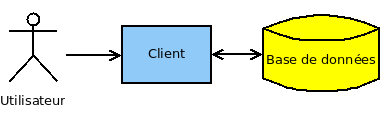
\includegraphics[scale=0.40]{acteurs}
  
  \begin{itemize}
   \item Communication avec Cassandra
   \item Evaluation des performances des algorithmes d'équilibrage de charge
  \end{itemize}

\end{frame}

\begin{frame}{Fonctionnement du projet}
\framesubtitle{Application cliente}
  \begin{block}{Initialisation}
    \begin{itemize}
    \item Connexion à la base de données
    \item Choix du keyspace
    \end{itemize}
  \end{block}

  \begin{block}{Console}
  L'utilisateur saisie la commande qu'il souhaite exécuter, notamment :
    \begin{itemize}
    \item Changement de keyspace
    \item Création de jeu de données
    \item Exécution d'un générateur de requêtes
    \end{itemize}
  \end{block}
\end{frame}

\begin{frame}{Axes de développement}
\begin{itemize}
	\item Base de données (\textit{Cassandra})
	\begin{itemize}
		\item Gestion des requêtes
		\item Gestion de la réplication
	\end{itemize}
	\item Application cliente (\textit{Driver Java Cassandra})
	\item Visualisation (\textit{Graphite})
\end{itemize}
\end{frame}


\section{Cassandra}

\begin{frame}{Base de données Cassandra}
\begin{textblock*}{\paperwidth}(-10pt,20pt)
    \raggedleft 
\includegraphics[scale=0.2]{cassandra_logo}
\end{textblock*}
Originellement créée et développée par \textbf{Facebook} en 2008 (maintenant un projet de la \textbf{Fondation Apache}), elle possède comme caractéristique d'être :
\begin{itemize}
	\item NoSQL, orientée colonnes
	\item Open-source (licence Apache 2)
	\item Écrite en Java
	\item Décentralisée
\end{itemize}
\end{frame}


\begin{frame}{Le choix de Cassandra}
\begin{textblock*}{\paperwidth}(-10pt,20pt)
    \raggedleft 
\includegraphics[scale=0.2]{cassandra_logo}
\end{textblock*}
\begin{itemize}
	\item Open-source
	\item Développement actif
	\item Proche du projet à réaliser
	\item Connaissances dans l'équipe
\end{itemize}
\textbf{Solutions alternatives} : HBase, CouchBase, CouchDB, from scratch...
\end{frame}

\section{Fonctionnement}

\begin{frame}{Fonctionnement de Cassandra}
\textbf{Gestion des requêtes : affectation}
\begin{columns}
\begin{column}[c]{5cm}
\begin{block}{De base}
\begin{itemize}
	\item Envoi des requêtes de lecture pour certains noeuds
	\item Renvoi donnée complète pour une requête, \textit{digest} pour les autres
	\item Suppression de requête de lecture \color{FailedRed}{\textbf{impossible}}
\end{itemize}
\end{block}
\end{column}

\begin{column}[c]{5cm}
\begin{block}{Modifié}
\begin{itemize}
	\item[\success] Envoi des requêtes de lecture pour \textbf{tous} les noeuds
	\item[\success] Renvoi donnée complète pour \textbf{toutes} les requêtes
	\item[\success] Suppression de requête de lecture \color{SuccessGreen}{\textbf{possible}}
\end{itemize}
\end{block}
\end{column}
\end{columns}
\end{frame}

\begin{frame}{Fonctionnement de Cassandra}
\textbf{Gestion des requêtes : réaffectation}
\begin{columns}
\begin{column}[c]{5cm}
\begin{block}{De base}
\begin{itemize}
	\item Système \color{FailedRed}{\textbf{inexistant}}
\end{itemize}
\end{block}
\end{column}

\begin{column}[c]{5cm}
\begin{block}{Modifié}
\begin{itemize}
	\item[\success] Compteur de requêtes assignées
	\item[\fail] Algorithmes d'assignation
	\item[\fail] Assignation
\end{itemize}
\end{block}
\end{column}
\end{columns}
\end{frame}

\begin{frame}{Fonctionnement de Cassandra}
\textbf{Gestion de la réplication}
\begin{columns}
\begin{column}[c]{5cm}
\begin{block}{De base}
\begin{itemize}
	\item Placement des copies d'un objet sur les noeuds suivant dans l'ordre du cercle
\end{itemize}
\end{block}
\end{column}

\begin{column}[c]{5cm}
\begin{block}{Modifié}
\begin{itemize}
	\item[\success] Placement des copies suivant différentes fonctions de hachages
\end{itemize}
\end{block}
\end{column}
\end{columns}
\end{frame}

%Pour expliquer la diapo précédente, présentation de stratégie simple (celle qui choisit les N noeuds suivants + celle qu'on doit implémenter
\begin{frame}{Fonctionnement de Cassandra}
\textbf{Stratégie de réplication de base}
\centering
    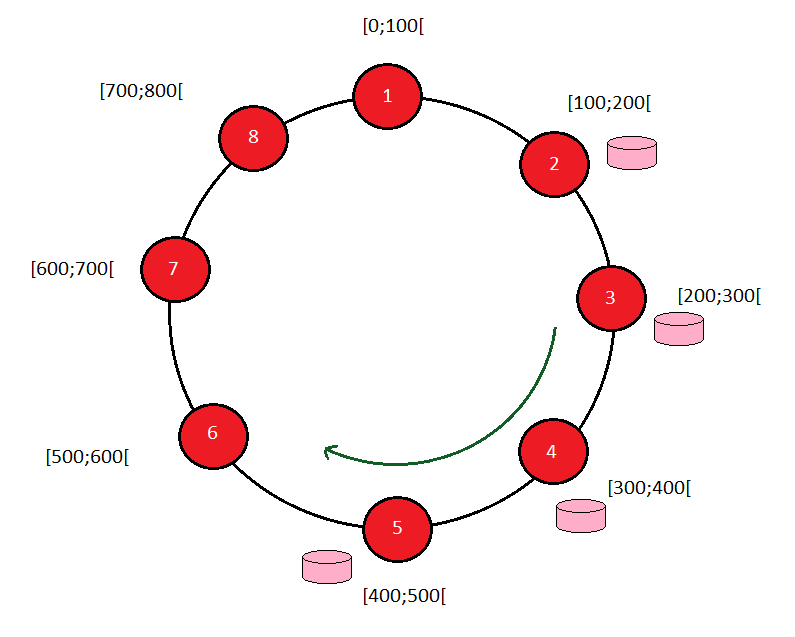
\includegraphics[scale=0.4]{replication}
\end{frame}

%Présentation des formules + dire ce que ça apporte (répartition de charge)
\begin{frame}{Fonctionnement de Cassandra}
\begin{columns}
\begin{column}[c]{5cm}
\begin{block}{De base}
\begin{itemize}
    \item Système \color{FailedRed}{\textbf{inexistant}}
\end{itemize}
\end{block}
\end{column}

\begin{column}[c]{5cm}
\begin{block}{Modifié}
\begin{itemize}
	\item[\fail] Gestion de la popularité
\end{itemize}
\end{block}
\end{column}
\end{columns}

\begin{block}{Paramètres}
    $r$ = Nombre de requêtes total effectuées durant l'intervalle de temps $T$; \newline
    $n$ = Nombre de noeuds dans le réseau; \newline
    $p$ = Popularité d'un objet; \newline
    $k$ = Nombre de copies de l'objet.
\end{block}

\begin{itemize}
    \item Augmenter le nombre de copies si $ 2 \times \frac{r}{n} \geq \frac{p}{k} $ vraie.
    \item Diminuer le nombre de copies si $ \frac{r}{2n} \leq \frac{p}{k} $ vraie.
\end{itemize}
\end{frame}


\section{Architecture}

\begin{frame}{Architecture de Cassandra}
\begin{block}{Staged event-driven architecture (SEDA)}
\begin{itemize}
    \item \textbf{Stage} $\rightarrow$ emplacement pour réaliser des tâches
    \begin{itemize}
	    \item \textbf{File d'attente} $\rightarrow$ messages de tâches à traiter
	    \item \textbf{Threads} $\rightarrow$ exécuteurs de tâches
    \end{itemize}
\end{itemize}
\end{block}
\centering
	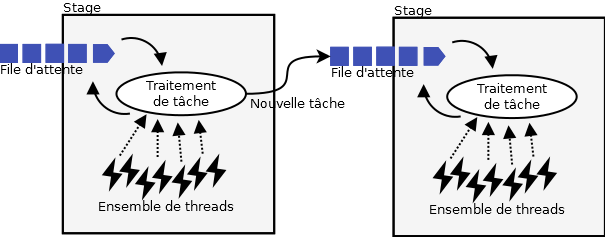
\includegraphics[scale=0.42]{stages}
\end{frame}

\begin{frame}{Architecture de Cassandra}
\begin{block}{Staged event-driven architecture (SEDA)}
\begin{itemize}
    \item \textbf{Stage} $\rightarrow$ emplacement pour réaliser des tâches
    \begin{itemize}
	    \item \textbf{File d'attente} $\rightarrow$ messages de tâches à traiter
	    \item \textbf{Threads} $\rightarrow$ exécuteurs de tâches
    \end{itemize}
\end{itemize}
\end{block}
Stages présents dans Cassandra :
\begin{itemize}
	\item READ
	\item \textbf{READ\_REMOVE}
	\item MUTATION
	\item GOSSIP
	\item ...
\end{itemize}
\end{frame}

\section{Points techniques}

% Présentation différences entre stratégie initialement souhaitée et celle implémentée, les conséquences et ce qu'il faut relativiser.
\begin{frame}{Point technique : Réplication}
\centering
    \begin{tabular}{| c | c | c | c |}
       \hline
       \rowcolor{UPMCEngagementBlueB} \multicolumn{2}{|c|}{Solution initiale}  & \multicolumn{2}{c|}{Solution implémentée} \tabularnewline
       \hline
       \rowcolor{UPMCEngagementBlueA} Donnée \no 1 & Donnée \no 2 & Donnée \no 1 & Donnée \no 2 \tabularnewline
       \hline
       $ H_0 (c1) $ & $ H_0 (c2) $ & $ H_0 (c1) $ & $ H_0 (c2) $  \tabularnewline
       \hline
       \rowcolor{UPMCEngagementBlueA} \multicolumn{4}{|c|}{1er réplica} \tabularnewline
       \hline
       $ H_1 (c1) $ & $ H_1 (c2) $ & $ H_1 (H_0 (c1)) $ & $ H_1 (H_0 (c2)) $  \tabularnewline
       \hline
       \rowcolor{UPMCEngagementBlueA} \multicolumn{4}{|c|}{2nd réplica} \tabularnewline
       \hline
       $ H_2 (c1) $ & $ H_2 (c2) $ & $ H_2 (H_0 (c1)) $ & $ H_2 (H_0 (c2)) $  \tabularnewline
       \hline
    \end{tabular}
\end{frame}

\section{Application cliente}
\begin{frame}{Application cliente}

\begin{block}{Technologies employées}
\begin{itemize}
    \item Développé en Java
    \item Utilisation d'un pilote informatique
\end{itemize}
\end{block}

\begin{block}{Pilote utilisé}
\begin{itemize}
    \item DataStax Java Driver 2.0
    \item Développé par l'entreprise DataStax
    \item Communication avec la base de données Cassandra
\end{itemize}
\end{block}


\end{frame}

\begin{frame}{Architecture du client}
\begin{textblock*}{\paperwidth}(10pt,50pt)
    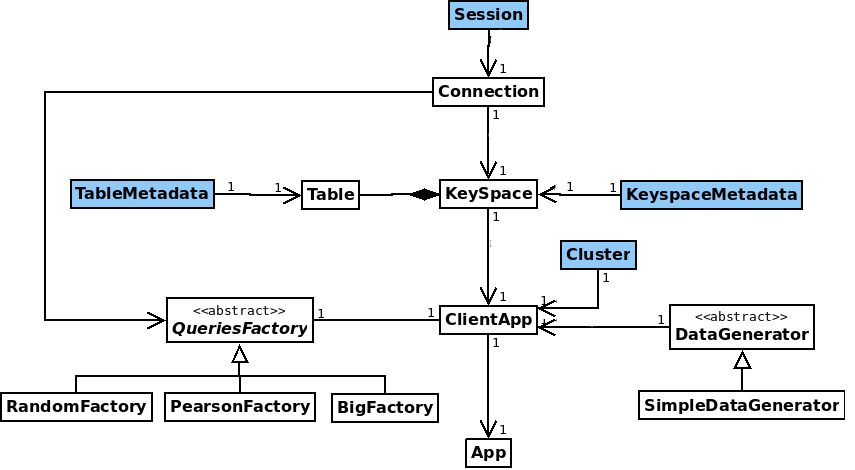
\includegraphics[scale=0.4]{architecture_client}
\end{textblock*}
\end{frame}



\begin{frame}{Fonctionnement du client}
\centering
    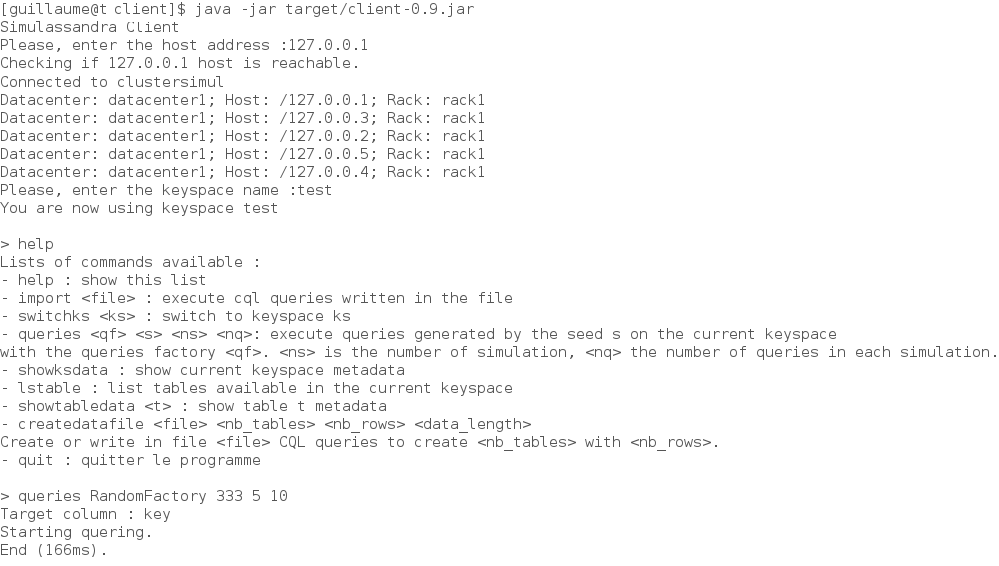
\includegraphics[scale=0.40]{captureclient}
\end{frame}

\begin{frame}{Générateur de requêtes}
\centering
    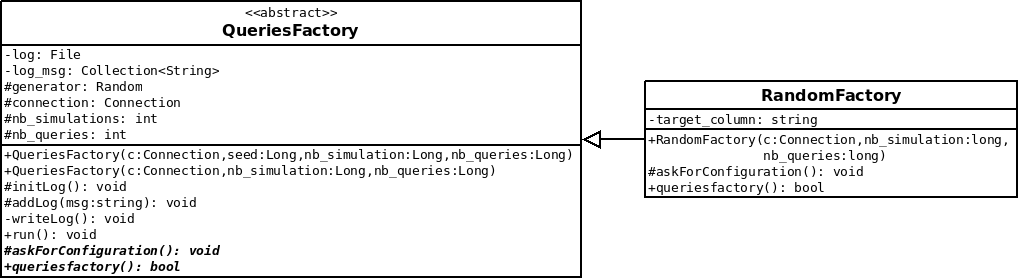
\includegraphics[scale=0.3]{architecture_req}


  \begin{block}{Personnalisable}
   \begin{itemize}
    \item Possibilité d'ajouter des générateurs de requêtes
    \item Choix du générateur \newline \texttt{queries NomGenerateur <seed> <nb\_simulations> <nb\_requetes>}
   \end{itemize}
  \end{block}
\end{frame}

\begin{frame}{Tests}
 \framesubtitle{Sur l'application cliente}
 \begin{block}{Tests }
	\begin{itemize}
	\item Tests unitaires
	\item Tests fonctionnels réalisés à la main
	\end{itemize}
 \end{block}
  
 \begin{block}{Améliorations souhaitées}
 	\begin{itemize}
 		\item Tests fonctionnels automatisés avec Cassandra
 		\item Tests unitaires 
 	\end{itemize}
 \end{block}
 
\end{frame}

% Présentation des 3 courbes, explications des résultats obtenus + une diapo récapitulant les acronymes.
\section{Tests}

\begin{frame}{Tests}
\framesubtitle{Sur Cassandra}
\begin{block}{Environnement}
    \begin{itemize}
        \item Les tests de mesures de performances se déroulent dans un réseau d'Amazon EC2 de 10 noeuds (machines dans le cloud) louées par le client.
        \item La base de données est composée de 10 000 objets de taille unique.
    \end{itemize}
\end{block}
\begin{block}{Dénomination}
    \begin{itemize}
        \item RF = nombre de copies + donnée originale
        \item petits objets = un texte généré aléatoirement de 10 Ko
        \item gros objets = un texte généré aléatoirement de 1 Mo
    \end{itemize}
\end{block}
\end{frame}

\begin{frame}{Tests}
\framesubtitle{Sur Cassandra modifiée}
\centering
    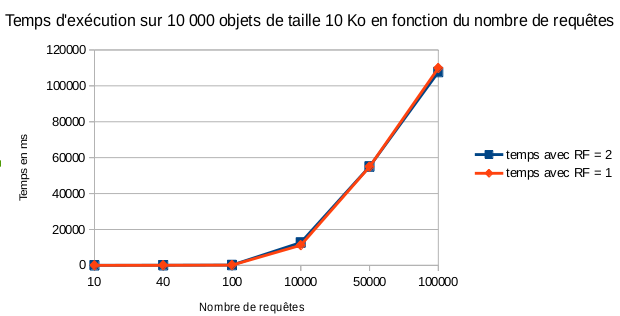
\includegraphics[scale=0.6]{PAF-RF-PO} \\
    \textbf{Gain : 2.4\% avec 100 000 requêtes = pas exhaustif}
\end{frame}

\begin{frame}{Tests}
\framesubtitle{Sur Cassandra non modifiée}
\centering
    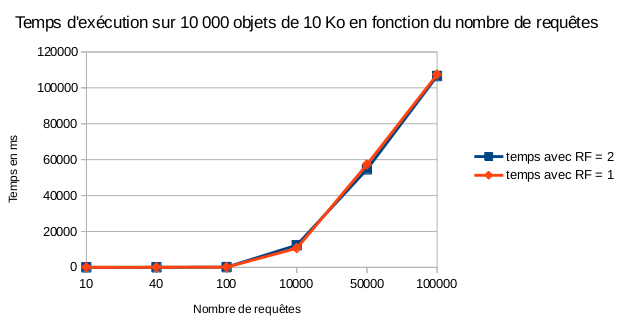
\includegraphics[scale=0.6]{cassandra_non_modif-RF-PO} \\
    \textbf{Gain : 0.77\% avec 100 000 requêtes = pas exhaustif}
\end{frame}


\begin{frame}{Tests}
\framesubtitle{Cassandra modifiée vs Cassandra non modifiée}
\centering
    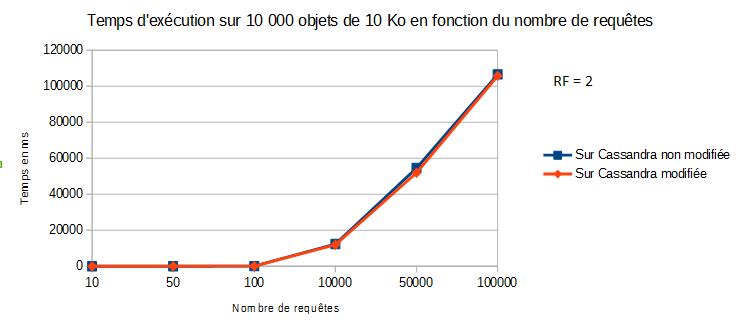
\includegraphics[scale=0.6]{PAF-CNMCM-RF2PO} \\
    \textbf{Gain : 0.73\% avec 100 000 requêtes = Trop petits objets ?}
\end{frame}


\begin{frame}{Tests}
\framesubtitle{Sur Cassandra modifiée}
\centering
    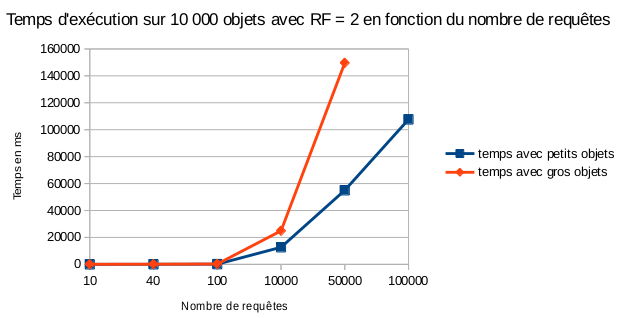
\includegraphics[scale=0.6]{PAF-TailleO-RF2} \\
    \textbf{Écart : 187\% avec 50 000 requêtes = Refaire les tests sur de gros objets}
\end{frame}


\section{Améliorations}

\begin{frame}{Perspectives}

\begin{block}{Cassandra}
\begin{itemize}
	\item Gestion des requêtes
	\begin{itemize}
		\item Algorithmes de réaffectation SVLO et AverageDegree
	\end{itemize}
	\item Gestion de la popularité
	\item Tests unitaires poussés
\end{itemize}
\end{block}
\begin{block}{Application client}
\begin{itemize}
	\item Meilleure ergonomie
	\item Amélioration des tests
\end{itemize}
\end{block}
\begin{block}{Visualisation}
\begin{itemize}
	\item Véritable logiciel de vue de performance
	\item Performance du réseau
\end{itemize}
\end{block}
\end{frame}

\mode<all>{ 
\SlideTransition{Questions ?}
}

% that's all folks
\end{document}
